\documentclass{beamer}
\usepackage{graphicx}
\usepackage{amsmath}
\usepackage{hyperref}
\usetheme{Madrid}
\usecolortheme{beaver}
\title{Simulation Based Inference using Marginal Neural Ratio Estimation}
\author{Gianmarco Puleo}
\date{SISSA, March 26th, 2025}

\begin{document}

\frame{\titlepage}

\begin{frame}{Summary and Goals}
    Given an observation of some data generated from the model
    \begin{equation}
        d_i = A \cos (\omega t_i + \phi) + \epsilon_i, \quad \epsilon_i \sim \mathcal{N}(0, \sigma^2)\label{eq:model}
    \end{equation}
    , we want to estimate the posterior 
    \begin{equation}
        p(\theta | x) = \frac{\mathcal{L}(\theta, x) \pi(\theta)}{p(x)} = r(\theta, x) \pi(\theta)
    \end{equation}
    \\
    where $\mathcal{L}(\theta, x)$ is the likelihood, $\pi(\theta)$ is the prior and $p(x)$ is the evidence.
    We present two ways of doing it:
    \begin{enumerate}
        \item Markov Chain Monte Carlo (MCMC)
        \item Simulation Based Inference (SBI) via Neural Ratio Estimation (NRE)
    \end{enumerate}
\end{frame}

\begin{frame}{Markov Chain Monte Carlo (Metropolis-Hastings)}
    We build a Markov chain of parameter samples, such that its limit distribution is the posterior. \\
    \textbf{Sketch of the algorithm:}
    \begin{enumerate}
        \item Initialise parameters $\theta_0$
        \item Generate a proposal next state $\theta^*$ from a proposal distribution $q(\theta^* | \theta_0)$
        \item Accept it with probability
        \[ P(\text{accept}) = \min\left(1, \frac{p(\theta^*) p(x | \theta^*)}{p(\theta_0) p(x | \theta_0)} \right) \]
        \item Repeat by generating a proposal from the current state.
    \end{enumerate}
    *For simplicity, assume a symmetric proposal and a uniform prior.
\end{frame}

\begin{frame}{Issues with MCMC}
    \begin{itemize}
        \item One should discard burn-in time and thin the chain by the autocorrelation time…
        \item The bottleneck is the repeated evaluations of the likelihood, which can be costly.
        \item In some cases, the likelihood is not even known in closed form!
    \end{itemize}
\begin{block}{Simulation Based Inference to the rescue}
    Assume we have a simulator $S:\theta \to d$ that generates data $d$ from known parameters $\theta$. 
    Neural Ratio Estimation uses $S$ to let a neural network learn the likelihood-to-evidence ratio $r(\theta, x) = p(x | \theta)/p(x)$.
    To this end we need to define:
    \begin{enumerate}
        \item A dataset
        \item A task (i.\ e.\ , a loss function)
        \item A model architecture
    \end{enumerate}
\end{block}
\end{frame}
\begin{frame}{Neural Ratio Estimation: the dataset}
    The \textbf{dataset} is generated as follows
        \begin{itemize}
            \item Generate $x_i = (\theta_i,d_i)$ pairs from the joint distribution $p(\theta, d)$, by sampling $\theta_i \sim \pi(\theta)$ and simulating $d_i = S(\theta_i)$.
            \item Scramble the pairs by randomly permuting the parameter instances, resulting in samples from the marginal distribution $p(d)p(\theta)$.
            \item To each pair, associate a binary label $C_i = 1$ if the pair is scrambled and $C_i = 0$ if it is not.
        \end{itemize}
    
    \begin{alertblock}{Goal}
        It can be shown that 
        \[p(C_i=1 | x_i) = \frac{1}{1+r(\theta_i, d_i)}.\]
        \[ \implies \text{ we want to perform a classification task!}\]
    \end{alertblock}
\end{frame}
\begin{frame}{Neural Ratio Estimation: the loss function}
    Let $f_\phi(\theta)$ be the neural network output with trainable parameters $\phi$.
    It is trained by minimising the binary cross-entropy loss with gradient descent:
    \begin{equation}
        \mathcal L(\phi) = -\frac{1}{N} \sum_{i=1}^N \Bigg\{ C_i \log \sigma(f_\phi(x_i)) + (1-C_i) \log\sigma(1-f_\phi(x_i)) \Bigg\}
    \end{equation}
    where $\sigma$ is the sigmoid function.
     
    NRE is enabled by the following equality:
        \begin{equation}
            \sigma(f_\phi(x)) = \frac{1}{1 + \exp(-f_\phi(x))}  \approx p(C_i=1 | x_i) = \frac{1}{1+r(\theta_i, d_i)}
        \end{equation}
    \pause
    \begin{equation}
        \implies f_\phi(x) \approx -\log(r(\theta_i, d_i)) .
    \end{equation}
\end{frame}
\begin{frame}{Model Architecture}
We actually want all 1-dimensional and 2-dimensional marginal posteriors. This suggests the following architecture: 
\begin{figure}
    \centering
    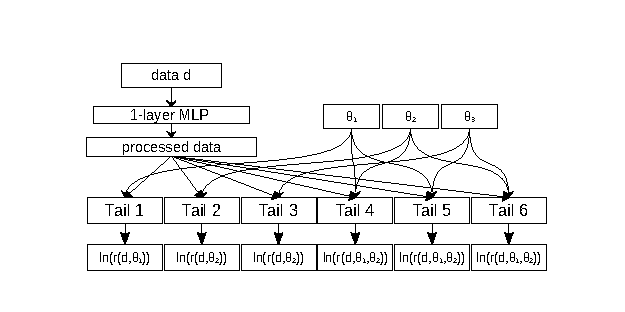
\includegraphics{nn_drawing.pdf}
    \caption{Neural network architecture for marginal NRE. The tails are fully connected layers.}
    \label{fig:architecture}
\end{figure}
\end{frame}
\begin{frame}[fragile]{Training technicalities}
\begin{itemize}
    \item the data were generated by equation \eqref{eq:model} with $\sigma = 0.1$ at $10$ evenly spaced time steps $t_i \in [0, 1]$. 
    \item The priors for the parameters are uniform distributions:
        \begin{equation}
            \omega \sim \mathcal{U}(2, 4), \quad \phi \sim \mathcal{U}(0, 6.28), \quad A \sim \mathcal{U}(0.5, 1.5).
        \end{equation}
    \item the total number of trainable parameters is 6286.
    \item I used the Adam optimizer with learning rate $10^{-3}$ and SGD with batches of 100 samples. I used a dataset of $10^6$ samples to train. 
          A validation set was used to monitor the training and for early stopping.
    \item The training took approximately one hour on my laptop (no GPU).
    \item I used \verb|lightning| and \verb|PyTorch| for model training. The code is available at 
          \href{https://github.com/g-puleo/bayes-i-exam.git}{https://github.com/g-puleo/bayes-i-exam.git}.
\end{itemize}
\end{frame}
\begin{frame}[allowframebreaks]{Results: marginal posteriors}
In order to plot the posterior distribution for some fixed observation $d_{\rm obs}$:
\begin{itemize}
    \item  sample parameters $\theta_i$ from the priors, 
    \item and then we reweight them by the NRE estimates of the likelihood-to-evidence ratio, 
    \[ w_i = \exp(-f_\phi(\theta_i, d_{\rm obs})) \].
\end{itemize}
This allows to produce histograms of the marginal posterior distributions.
\begin{columns}
    \begin{column}{0.7\textwidth}
        \begin{figure}
            \centering
            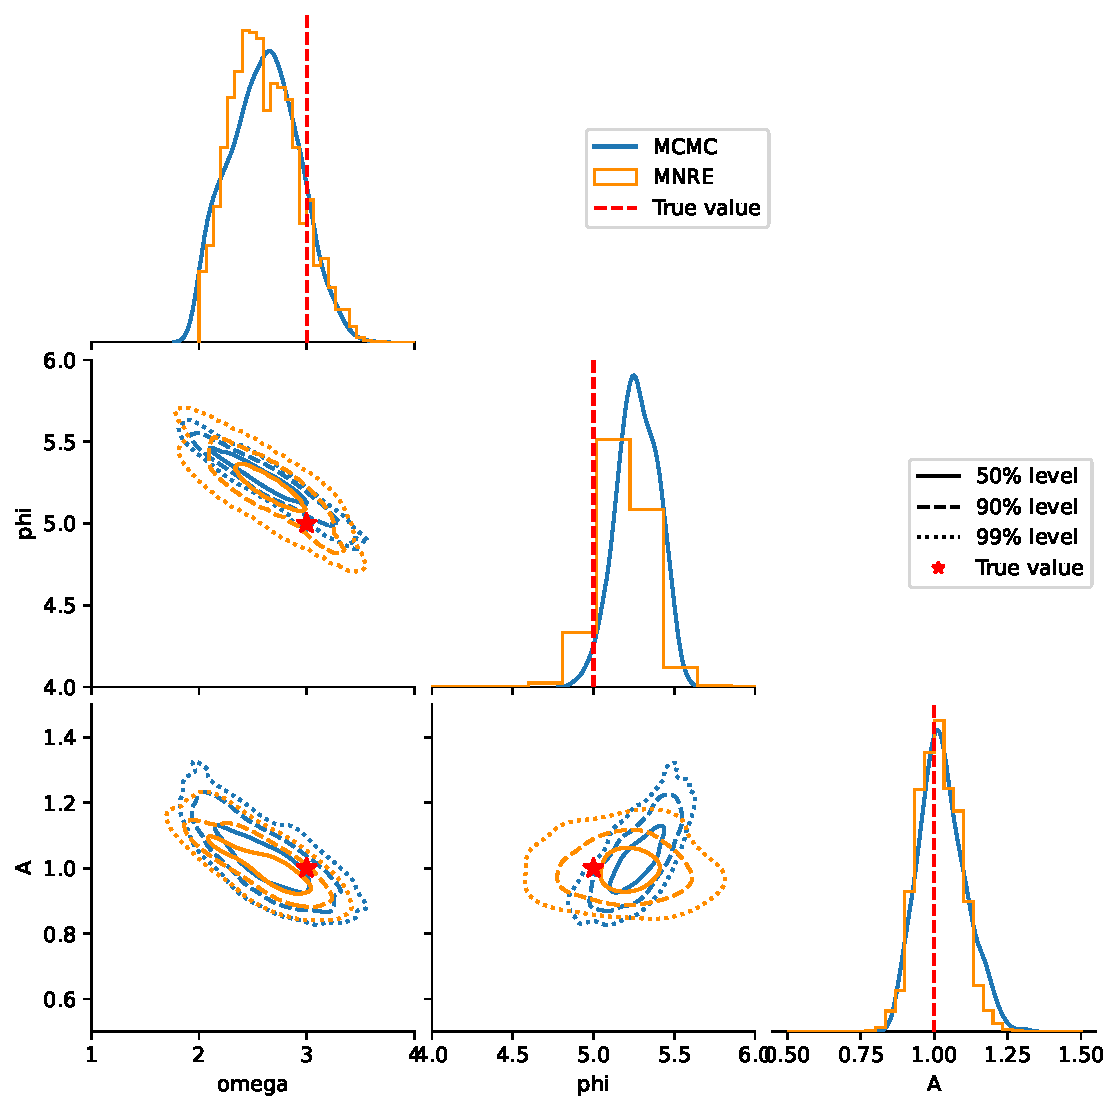
\includegraphics[height=0.8\textheight]{../figures/pairplot_mc_samples.pdf}
            \label{fig:marginal_posteriors}
        \end{figure}
    \end{column}
    \begin{column}{0.3\textwidth}
        Marginal posteriors for the parameters $\theta = (\omega, A, \phi)$. The blue lines are the MCMC posteriors, while the orange lines are the NRE estimates.
    \end{column}
\end{columns}
\end{frame}
\begin{frame}{Results: p-p plot}
    \begin{figure}
        \centering
        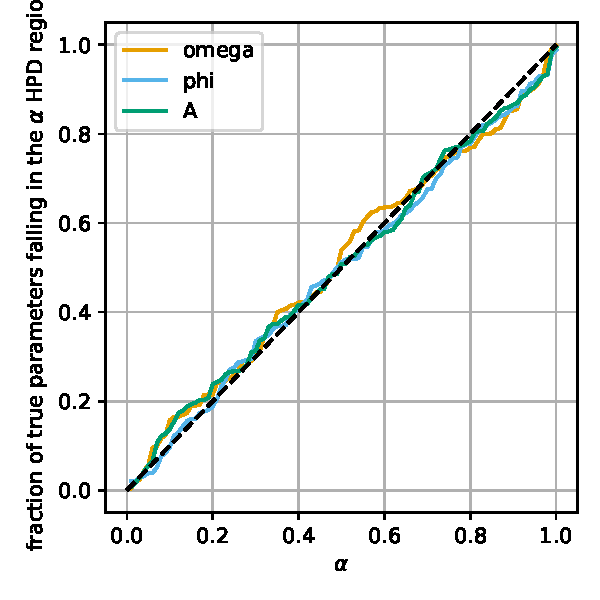
\includegraphics[height=0.7\textheight]{../figures/pp_plot_light_v2.pdf}
        \caption{P-P plot for the NRE estimates. For each parameter we are close to the diagonal.}
        \label{fig:pp_plot}
    \end{figure}
\end{frame}
\begin{frame}{Results: coverage map}
For each point in a ($A$, $\omega$) grid, we evaluate the coverage of the $\alpha$-HPD region of the posterior on a set of $1000$ observation from 
different $\phi$ values. 
    \begin{figure}
        \centering
        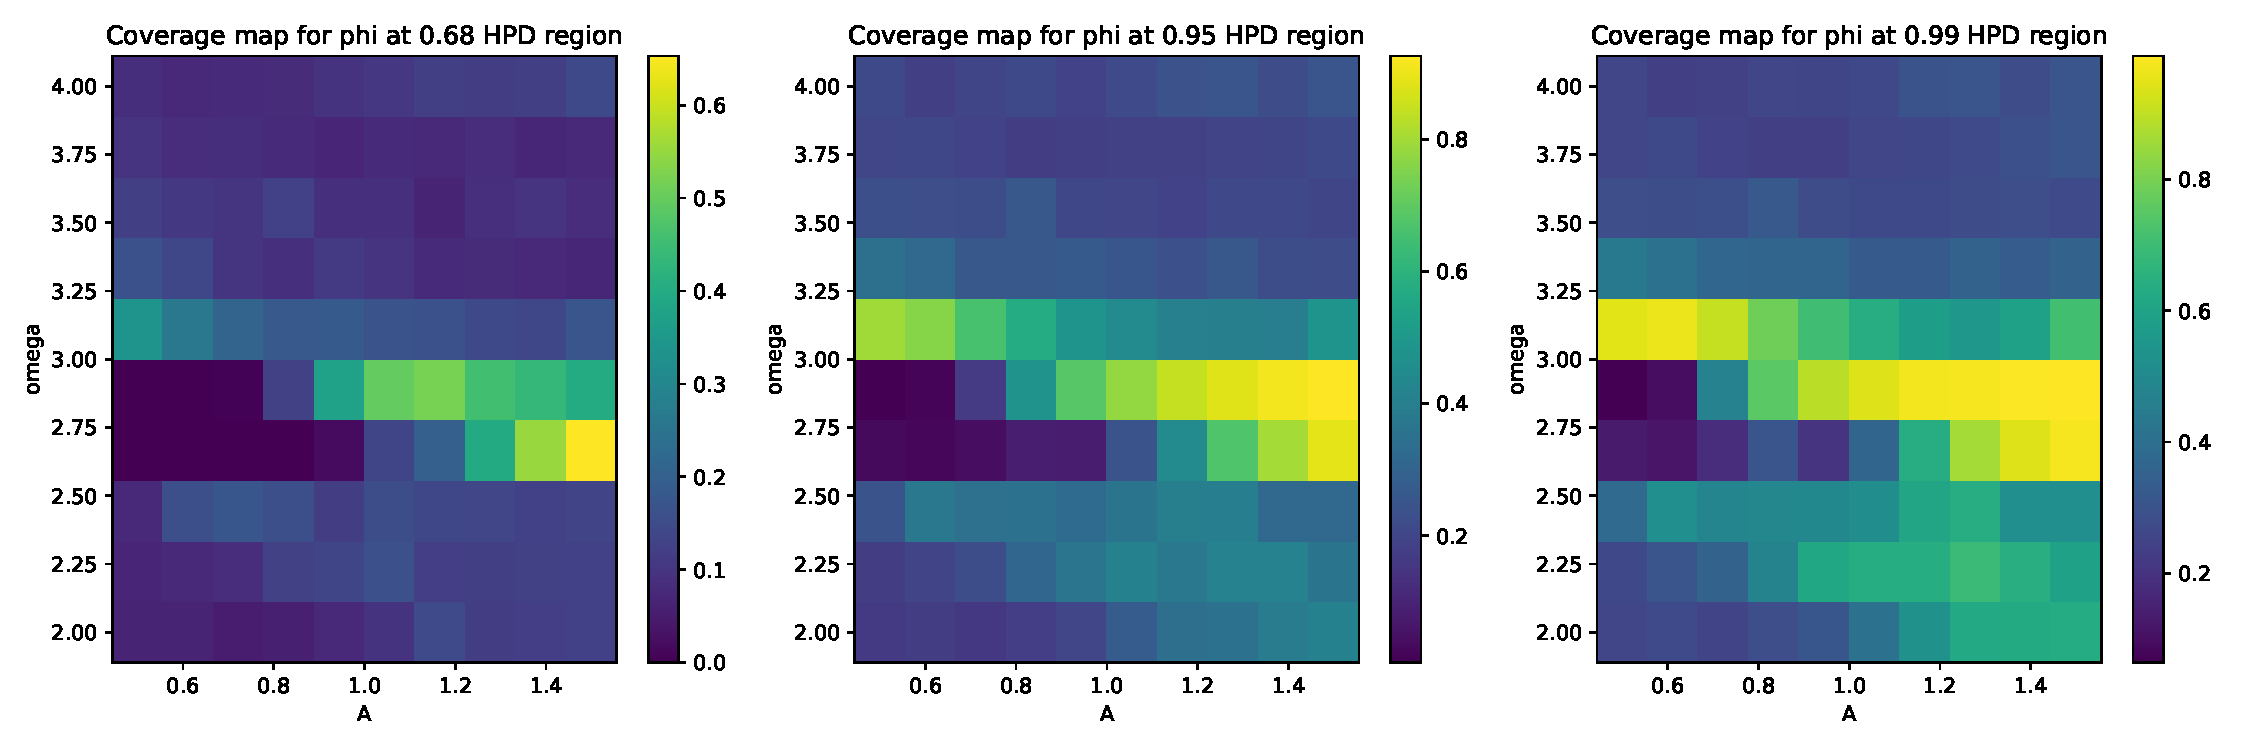
\includegraphics[width=\textwidth]{../figures/coverage_map_light_v2.pdf}
        \caption{Coverage map for the NRE estimates. The neural network does not seem optimal in all regions of the parameter space where it was trained.}
        \label{fig:coverage_map}
    \end{figure}
\end{frame}
\begin{frame}[fragile]{Conclusion}
    \begin{itemize}
        \item The trained NRE network can produce \textbf{amortized} estimates of the \textbf{posterior}, thus the likelihood costs are completely avoided.
        \item The model was implemented in a scalable and efficient way using \verb|PyTorch| and \verb|lightning|.
        \item The coverage of these posterior is optimal in some regions of parameter space.
        \item The reason for sub-optimal coverage properties in some regions might be linked to having a model with too few parameters for the amount of datapoints shown. 
        \item Future work could explore increasing model complexity to improve coverage in underperforming regions.
    \end{itemize}
\end{frame}
\end{document}
